\section[Scintillation detectors]{Scintillation detectors \label{sec:scintillators}}
There are two scintillator-based detectors deployed in the \gx{} spectrometer: a small barrel-shaped detector surrounding the
target, referred to as the Start Counter (ST), and a two-plane hodoscope detector system in the forward direction, referred to as the
Time-of-Flight (TOF) detector. Both detectors provide timing information. Charged-particle identification is derived from
energy loss ($dE/dx$) in the ST and flight time from the TOF.

\subsection{Start Counter \label{sec:st}}

The ST, shown in Fig.~\ref{fig:st-overview-drawing},
surrounds the target
region and covers about 90\% of the solid angle for particles
originating from the center of the target. The ST is designed to operate
at tagged photon beam intensities of up to $10^8$ photons per second
in the coherent peak, and has a high degree of segmentation to limit
the per-paddle rates. The time resolution must be sufficient to resolve the RF beam structure and identify the electron beam bunch from which the event originated
(see Section\,\ref{sec:ebeam}). The ST provides a timing signal that is relatively independent of particle type and trajectory (because of its proximity to the target) and can be used in the Level 1 trigger if necessary. The specific energy deposits dE/dx in ST are used for charged-particle identification in combination with the flight-time from the TOF.
Details of the design, construction and performance of the ST system can be found in 
Ref.\,\cite{Pooser:2019rhu}.

\begin{figure}[!htb]
\centering
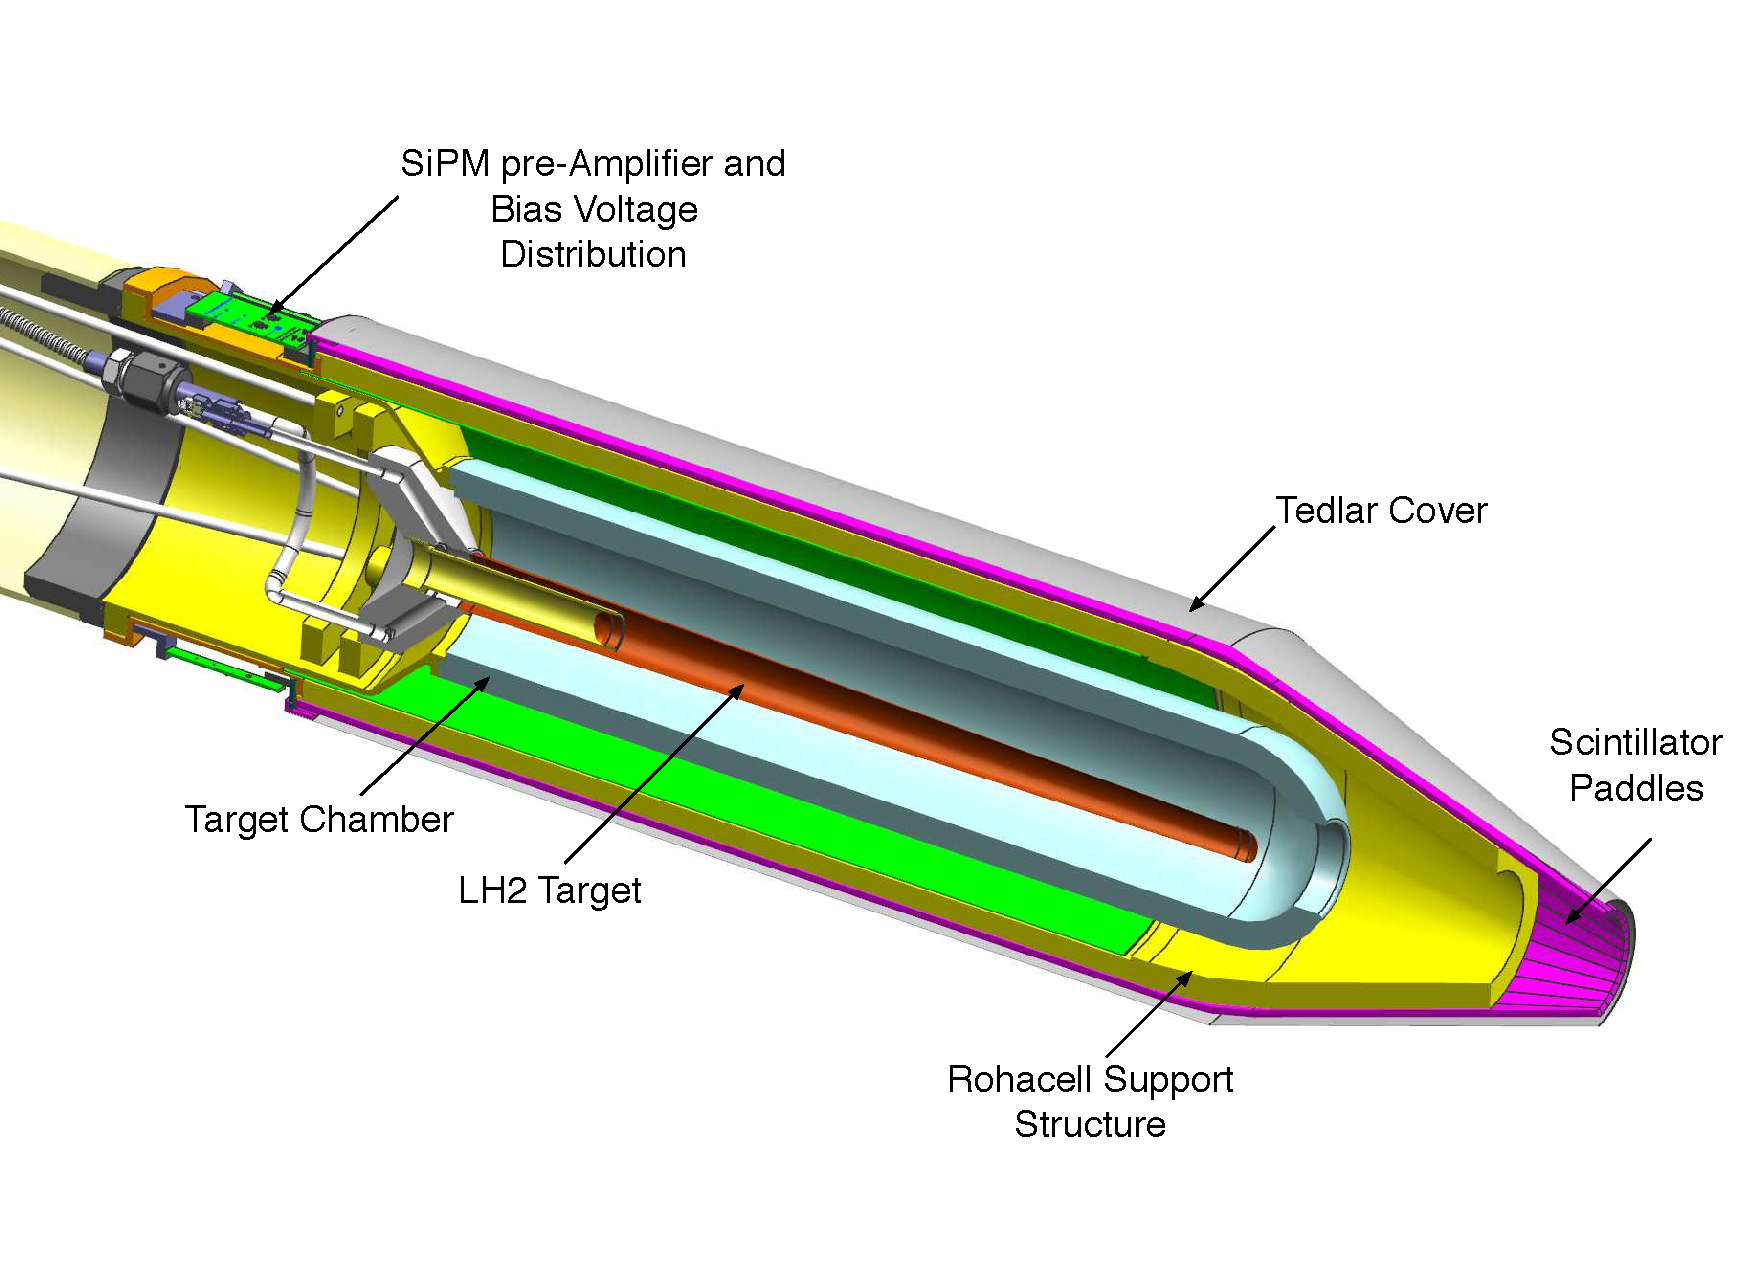
\includegraphics[width=1.0\columnwidth]{figures/start_counter_all.pdf}
\caption{The \gx{} Start Counter surrounding the liquid-hydrogen
  target assembly.  The incident beam travels from left to right down the central
  axis.\label{fig:st-overview-drawing}}
\end{figure}

The ST consists of 30 scintillator paddles arranged in a cylinder of radius 78~mm with a ``nose'' section that bends towards the beam
line to a radius of 20~mm at the downstream end. EJ-200 scintillator from Eljen
Technology\footnote{Eljen Technology, https://eljentechnology.com/products/plastic-scintillators.} was
selected for the ST paddles. EJ-200 has a decay time of 2.1~ns with a bulk attenuation length
of 380~cm. 
Each scintillator paddle originated from stock 3~mm thick and 600 mm in
length. The paddles were bent at Eljen to create the nose section, and then machined at McNeal Enterprises Inc.\footnote{McNeal
  Enterprises~Inc., http://www.mcnealplasticmachining.com} to their
final shape, including edges beveled at $6^\circ$ to minimize loss of
acceptance.
The scintillator paddles are supported by a Rohacell closed-cell foam
structure. The Rohacell is 11~mm thick and is rigidly attached to an
aluminum support hub at the upstream end. The downstream support
extends partially into the nose section. The cylindrical length of the Rohacell is further reinforced with three layers of carbon fiber, each layer being 650~$\mu$m thick. The assembly is made light-tight with a Tedlar wrapping, attached to a plastic collar at the upstream end.

Silicon photomultiplier detectors are used as light
sensors, as these are not affected by the magnetic field produced by the solenoid. The SiPMs were placed
at the upstream end of each scintillator element with a 250~$\mu$m air gap.
Each paddle is read out with an array of four 
SiPMs (Hamamatsu S109031-050P multi-pixel photon counters) whose signals are summed. 
The on-board electronics provides two signals per paddle, one delivered to an FADC, and the other to a 5$\times$~amplifier that is sent to a discriminator and then to a TDC. 
%The performance of the ST is discussed in section~\ref{sec:scperformance}.

\subsection[Time-of-Flight counters]{Time-of-flight counters \label{sec:tof}}
The TOF system delivers fast timing signals from charged particles passing through the detector thereby providing information for particle identification.
The TOF detector is a wall of scintillators located about 5.5~m downstream from the target, covering 
a polar angular region from 0.6$^{\circ}$ to 13$^{\circ}$. The detector has two planes of
scintillator paddles stacked in the horizontal and vertical direction. Most paddles are 252~cm long and 2.54~cm
thick with a width of 6~cm. 
The scintillator material is EJ-200 from Eljen Technology.
To allow the photon beam to pass through the central region,
an aperture of 12$\times$12\,cm$^2$ is kept
free of any detector material by using four shorter, single-PMT paddle detectors with a length of 120~cm around the beam hole
in each detector plane. These paddles also have a width of 6~cm and a thickness of 2.54~cm. In order to keep the
count rate of the paddles well below 2~MHz the two inner-most full-length paddles closest to the beam hole on either side have a reduced width of 3~cm.
Light guides built out of UV transmitting plastic provide the coupling between the scintillator and the PMT and allow the 
magnetic shielding to protect the photocathode by extending about 5~cm past the PMT entrance window. All paddles are wrapped
with a layer of a highly reflective material (DF2000MA from 3M) followed by a layer of strong black Tedlar film for light tightness. 

The scintillator paddles are read out using 
PMTs from Hamamatsu.\footnote{Hamamatsu Photonics, https://www.hamamatsu.com/us/en/index.html.} Full-length paddles
have a PMT at both ends, while the short paddles have a single PMT
at the outer end of the detector. These type H10534 tubes have ten stages and are complete assemblies with high voltage base, casing and $\mu$-metal shielding. Additional soft-iron external shielding protects each PMT from significant stray fields from the solenoid magnet.


\subsection{Electronics \label{sec:scelectronics}}
High voltage for the TOF PMTs is provided by CAEN HV modules of type A1535SN, initially controlled by a CAEN SY1527 main frame and
later upgraded to a SY4527.
The PMT outputs are connected to a passive splitter by a 55'-long RG-58 coaxial cables. The signal is split into two equal-amplitude signals. One signal is directly connected to a FADC~\cite{Dong:2007}, while the second signal passes first through a leading-edge discriminator and is then used as an input to a high resolution TDC. The digitizing modules are mounted in VXS crates as described in Section~\ref{sec:trig}.
The threshold of the leading-edge discriminator is controlled separately for each channel and has an intrinsic
deadtime of about 25~ns.

The sparcification threshold for the FADC is set to 120 (160) counts for the ST (TOF), with the nominal pedestal set at 100 counts. The high voltage of each TOF PMT is adjusted to generate the amplitude of the signal from a minimum-ionizing particle of at least 400 ADC counts above baseline. The data from the FADC is provided by the FPGA algorithm and consists
of two words per channel with information about pedestal, signal amplitude, signal integral, and timing.

The timing signals from the ST system are registered using the JLab F1 TDCs, which have a nominal least count of 58~ps. In order to take advantage of the higher intrinsic resolution of the TOF counters, this system uses the VX1290A TDCs from CAEN\footnote{CAEN, https://www.caen.it/}, which are multi-hit high-resolution TDCs with a buffer of up to 8 words per channel and a nominal least count of 25~ps. Since these TDCs provide the best time measurements in the \gx{} detector, the timing of the accelerator RF signal is also
digitized using these TDCs.

\subsection{Calibration and monitoring \label{sec:sccalib}}
The combined ST and TOF systems are used to determine the flight times of particles, the ST providing a precise start time in combination with the accelerator RF, and the TOF providing the stop time. Both systems may also be used to provide information on particle energy loss. Therefore, the signals in ST and TOF must be 
calibrated to determine corrections for the effects of
time-walk, light propagation time offsets, and light attenuation. The procedures are slightly different for the two detectors because of the different geometries, intrinsic resolutions, and the advantages of the TOF system having two adjacent perpendicular planes. 

For the time-walk correction for each paddle of the ST, the detector signal is sent to both an FADC and a TDC. The time from the FADC, being independent of pulse amplitude, is the reference. The amplitude dependence of the difference between TDC and FDC times is used to measure the time walk; the resulting curve is fit to an empirical function for use in the correction. 
The propagation time is measured as a function of the hit position in a paddle as determined by well-reconstructed charged particle tracks. The propagation velocity is measured in three regions of the counter (``straight,'' ``bend,'' and ``nose'') and is not assumed to be a single value for all hits. The light attenuation is also measured at several positions along the counter using charged particle tracks. The energy-per-unit pathlength in the paddle as a function of distance from the SiPM is fit to a modified exponential, with different parameters allowed for the straight section and the nose section, with continuity enforced at the section boundary.

The calibration procedures for the TOF system take advantage of the two
planes of narrow paddles oriented orthogonal to each other, which permits calibration of the full TOF detector independent
of any other external detector information. The overlap region of two full-length paddles from the two planes define
a 6$\times$6~cm$^2$ area for most paddles, with a few 3$\times$3~cm$^2$ areas close to the beam hole. The separation between the two detector planes is minimal as they are mounted adjacent to each other, separated only by wrapping
material. While the time-difference (TD) between the two ends of a paddle is related to the hit position along the paddle,
the mean-time (MT) is related to the flight time of a particle from the vertex to the paddle. Therefore, the MT for two overlapping
paddles must be the same when hit by the same particle passing through both paddles, while the hit position in the horizontal and vertical dimensions are defined by the TD of the two paddles. This relationship results in an internally consistent calibration of all paddles with respect to every other paddle. Prior to finding timing offsets for calibration, all times must corrected for the amplitude-dependent walk. The relation between time at threshold and signal amplitude is parameterized and used to correct for time slewing.

After all full-length paddles have been calibrated, they can be used themselves as references to
calibrate the remaining eight short paddles that only have single-ended readout.  Again we use the fact that any overlap region of two paddles from different
planes has the same particle flight time from the vertex. This coincidence produces peaks in the time difference distributions that can be used to determine the timing offsets of these single-ended readout paddles. 

To test the calibration, we take tracks that are incident on a paddle in one plane and compute the time difference between the MT of that paddle and the MT of every other full-length paddle in the other plane. The resulting distribution of these differences is shown in Fig.~\ref{fig:mt_diff}. Assuming that all paddles have the same timing resolution, we can compute the
average time resolution to be $\sigma$ = 105~ps$=\frac{148}{\sqrt{2}}$~ps, assuming a Gaussian distribution.
\begin{figure}[tbp]
\begin{center}
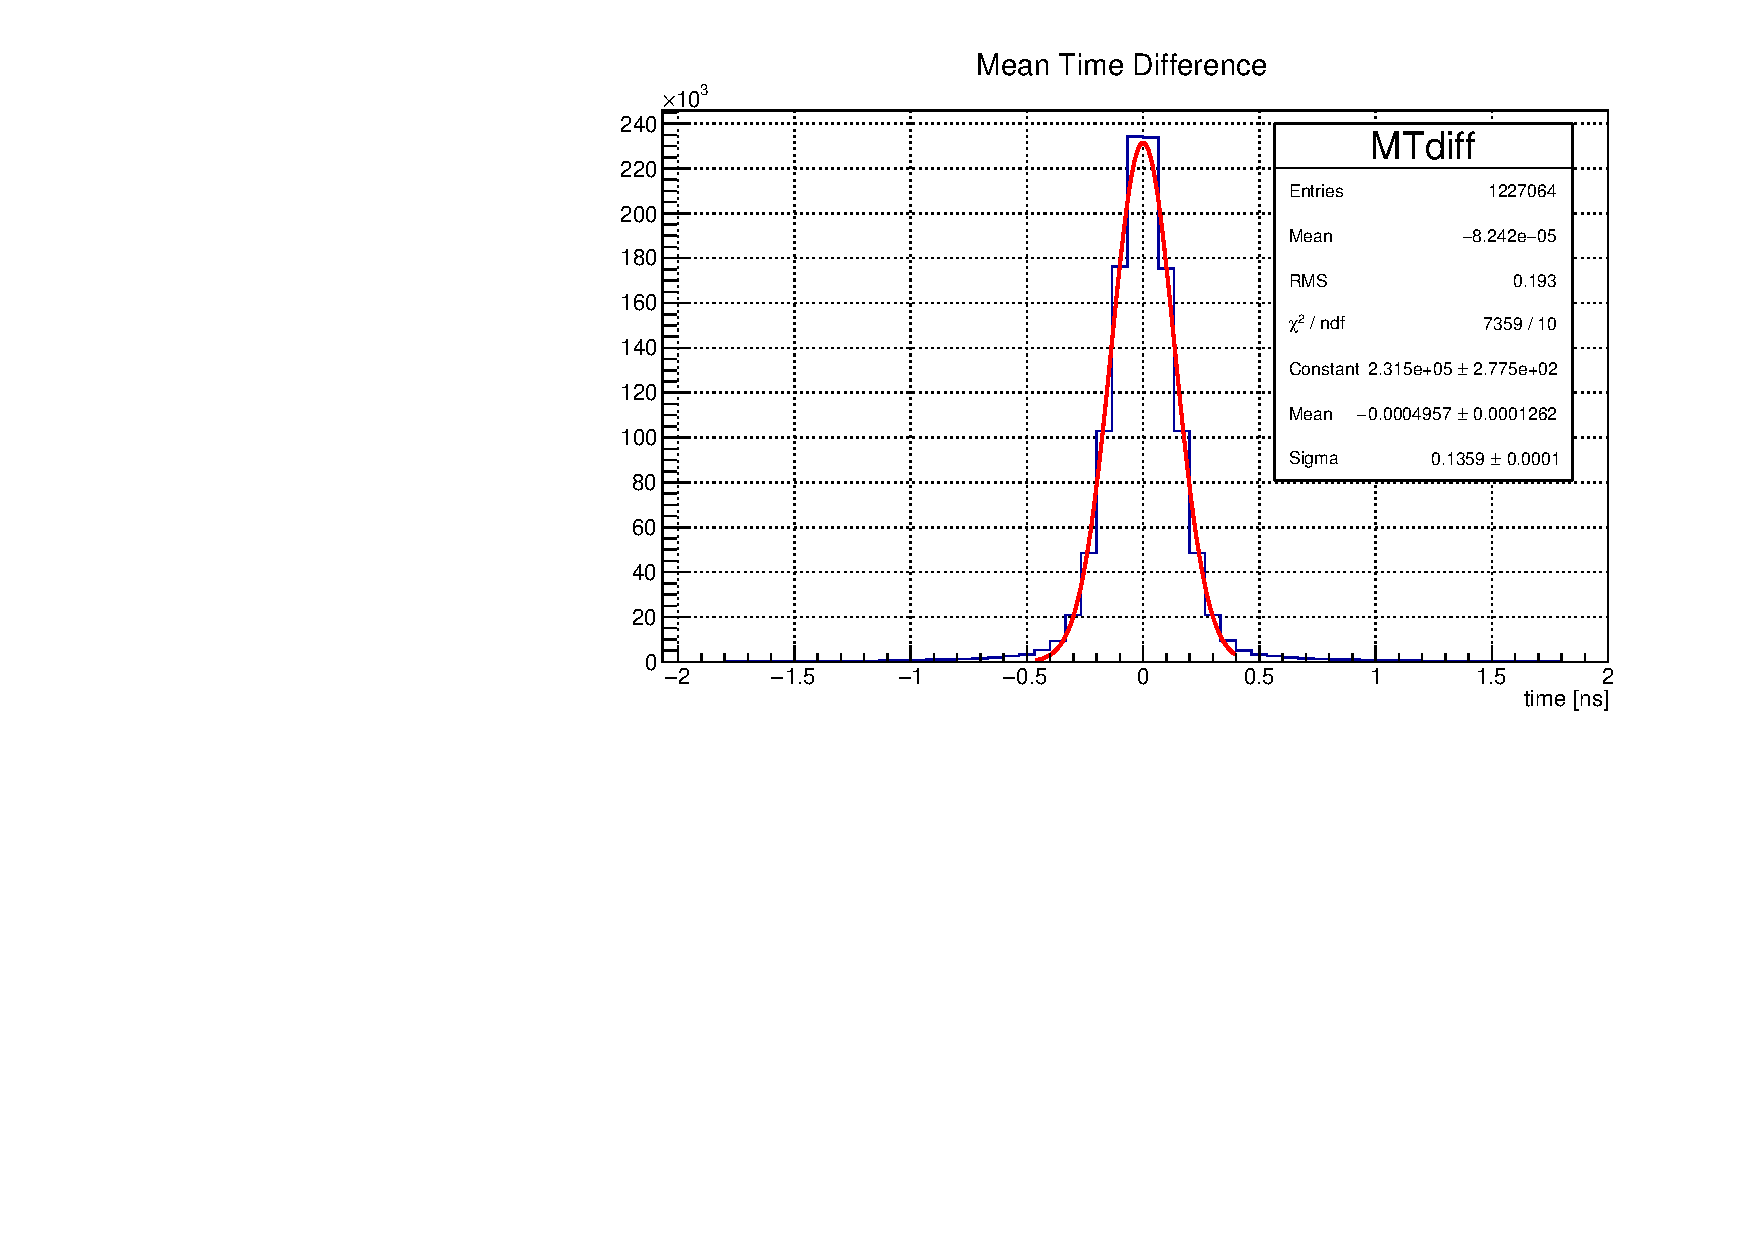
\includegraphics[width=0.6\textwidth]{figures/mt_diff_fullTOF.pdf}
\caption{\label{fig:mt_diff} Mean time difference between one TOF long paddle of one plane with all other long paddles
of the other plane. (Color online)}
\end{center}
\end{figure}

\subsection{Performance \label{sec:scperformance}}
The purpose of the ST is to select the correct beam bunch that generated an interaction in the target, which will be used to determine the event start time using the accelerator RF time. Therefore, the ST resolution does not contribute to the resolution of the flight time as long as the resolution is sufficient to pick out the correct beam bunch with high probability.

The ST timing performance can be measured by comparing the event time in the target as measured by the start counter and the time derived from a signal from the CEBAF accelerator, which is synchronized with the RF time structure of the machine. The start counter time must be corrected for the flight path of the charged particle emerging from the event, and all instrumental corrections mentioned in the previous section must be applied. Fig.~\ref{fig:st-time-resolution} shows the distribution of this time difference. The average time resolution is $\sigma$=234~ps, although the resolution varies depending on the position of the hit along the counter. 

%Table~\ref{table:st-time-resolution} gives the measured time resolution for the various sections as well as for all sections, with all paddles combined. Also shown is the fraction of tracks kept by a $\pm 1.0$~ns cut around the central value.

\begin{figure}[tbh]
  \centering
  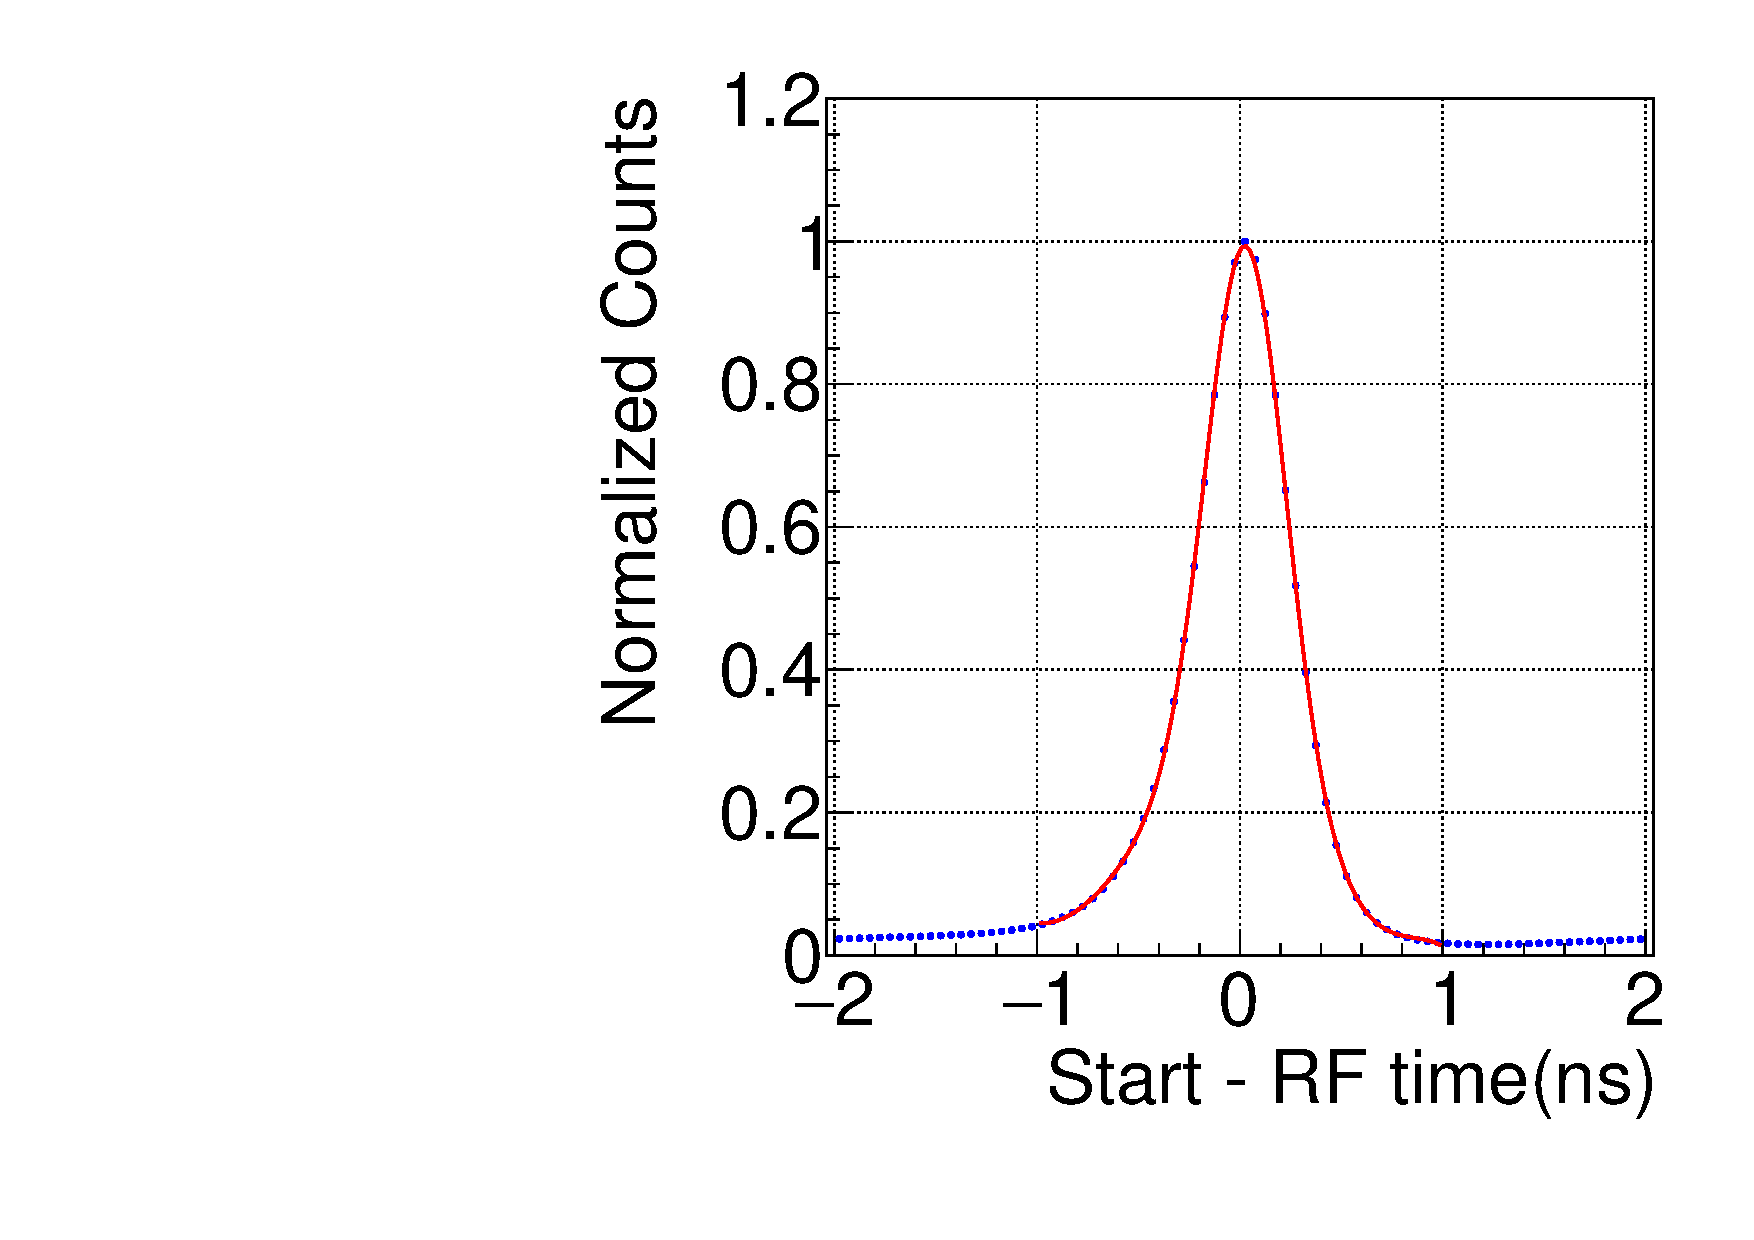
\includegraphics[width=0.6\linewidth]{figures/st_tr_fit.pdf}  
  \caption{Time difference distribution between the vertex time computed from the start counter and the accelerator RF. The time from the RF does not contribute significantly to the width of the distribution. The fit function is a double Gaussian plus a third-degree polynomial.
  %The vertical lines indicate the cuts used to identify a 250~MHz beam bunch.
  }
                \label{fig:st-time-resolution}
\end{figure}  

%\begin{table}[htbp]
%  \centering
%  \begin{tabular}{@{} l *4c @{}}
%    \hline
%    \multicolumn{1}{c}{\textbf{Section}}    & \textbf{All}  & %\textbf{Straight}  & \textbf{Bend}  & \textbf{Nose}  \\ 
%    \hline
%    $\mathbf{FWHM}$ & 550~ps & 690~ps & 700~ps & 450~ps \\ 
%    \textbf{Fraction} & 93\% & 92\% & 91\% & 94\% \\\hline
%  \end{tabular}
% \caption{Average time resolutions (FWHM) and event fractions within a 
% $\pm$ 1~ns window for all 30 ST sectors by independent geometrical regions.}
%  \label{table:st-time-resolution}
%\end{table}  

The ST can also be used to identify particles using $dE/dx$. Fig.~\ref{fig:ST_dEdx_vs_p} shows $dE/dx$ versus momentum, $p$,
for charged particles matched to the Start Counter. Protons can be
separated from pions up to $p=0.9$~GeV/$c$.

\begin{figure*}[!htb]
  \centering
  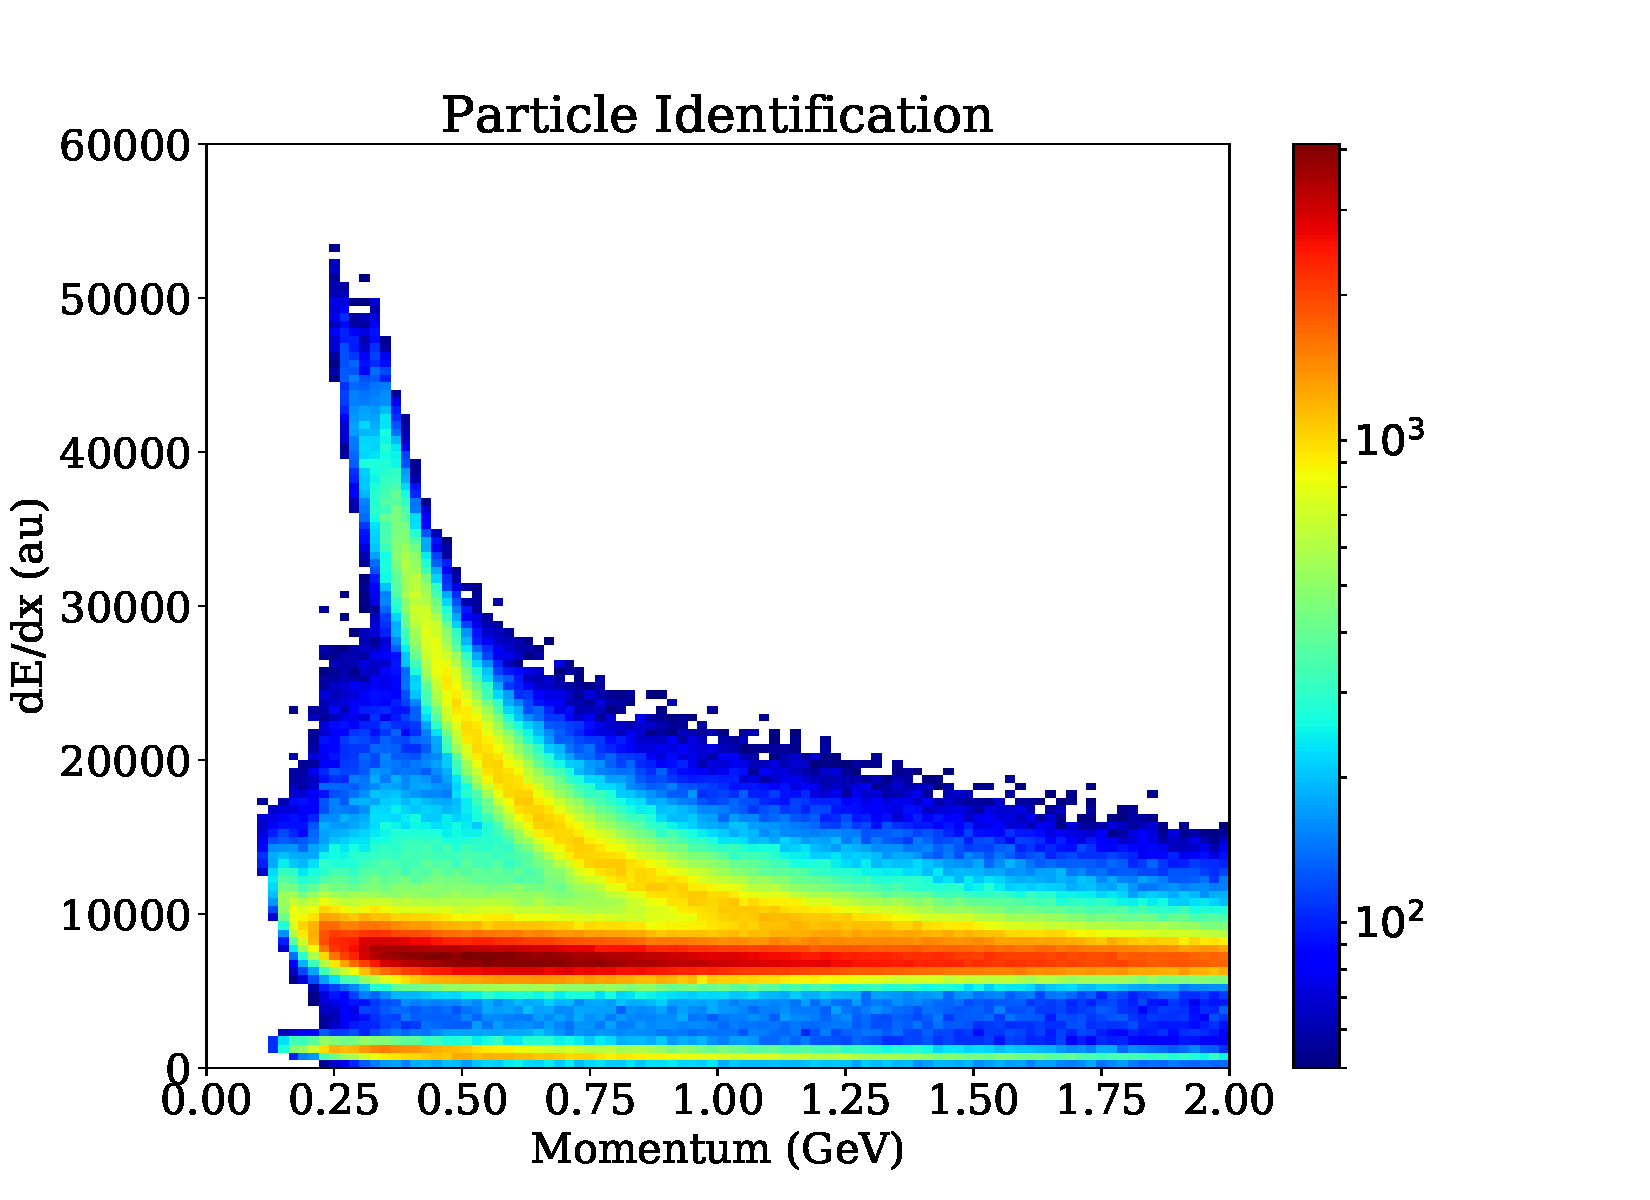
\includegraphics[width=0.6\textwidth]{figures/st_dedx_vs_p.pdf}
  \caption{$dE/dx$ vs.\ $p$ for the Start Counter.  The curved band
    corresponds to protons while the horizontal band corresponds to
    electrons, pions, and kaons. Pion/proton separation is achievable
    for tracks with $p < 0.9$~GeV/$c$.}\label{fig:ST_dEdx_vs_p}
\end{figure*}

The performance of the TOF detector for particle identification (PID) was investigated by considering the relative number of
particle types within the event sample. Events were selected with at least three fully-reconstructed positively-charged tracks, with at least one of these tracks intersecting the TOF detector. More pions are expected than protons, and more protons than kaons. Looking at the distribution of velocity, $\beta$, of these tracks as a function of momentum, the bands from protons, kaons and pions are easily identified (see Fig.~\ref{fig:betavsp}). 

The distributions of $\beta$ at two specific track momenta, 2~GeV/c and 4~GeV/c (see Fig.~\ref{fig:betaproj}), are illustrative of the PID capability of the TOF detector. At $p=2$~GeV/c, the TOF detector provides about a 4$\sigma$ separation between
the pion/positron peak and the kaon peak, sufficient to identify tracks as kaons with $\beta=0.97$, or lower, with very
high certainty. However, at  $\beta=0.98$, the probability of the track being a kaon is less than 50\%, due to the abundance of pions that is an order of magnitude larger than kaons. The protons, on the other hand, are very well
separated from the other particle types and can be identified with high confidence over the full range in $\beta$.
At a track momentum of 4~GeV/c, PID becomes much more difficult and represents the limit at which the TOF can identify protons with high confidence. The separation between the large peak containing pions, kaons and positrons from the proton
peak is about 4$\sigma$, while the relative abundance in this case is about a factor of 4. As a consequence, a 4~GeV/c momentum
track with $\beta=0.975$ is most likely a proton, with a small probability of being a pion. At $\beta=0.98$, such
a track has a similar probability for being a proton or a pion.
\begin{figure}[tbp]
\begin{center}
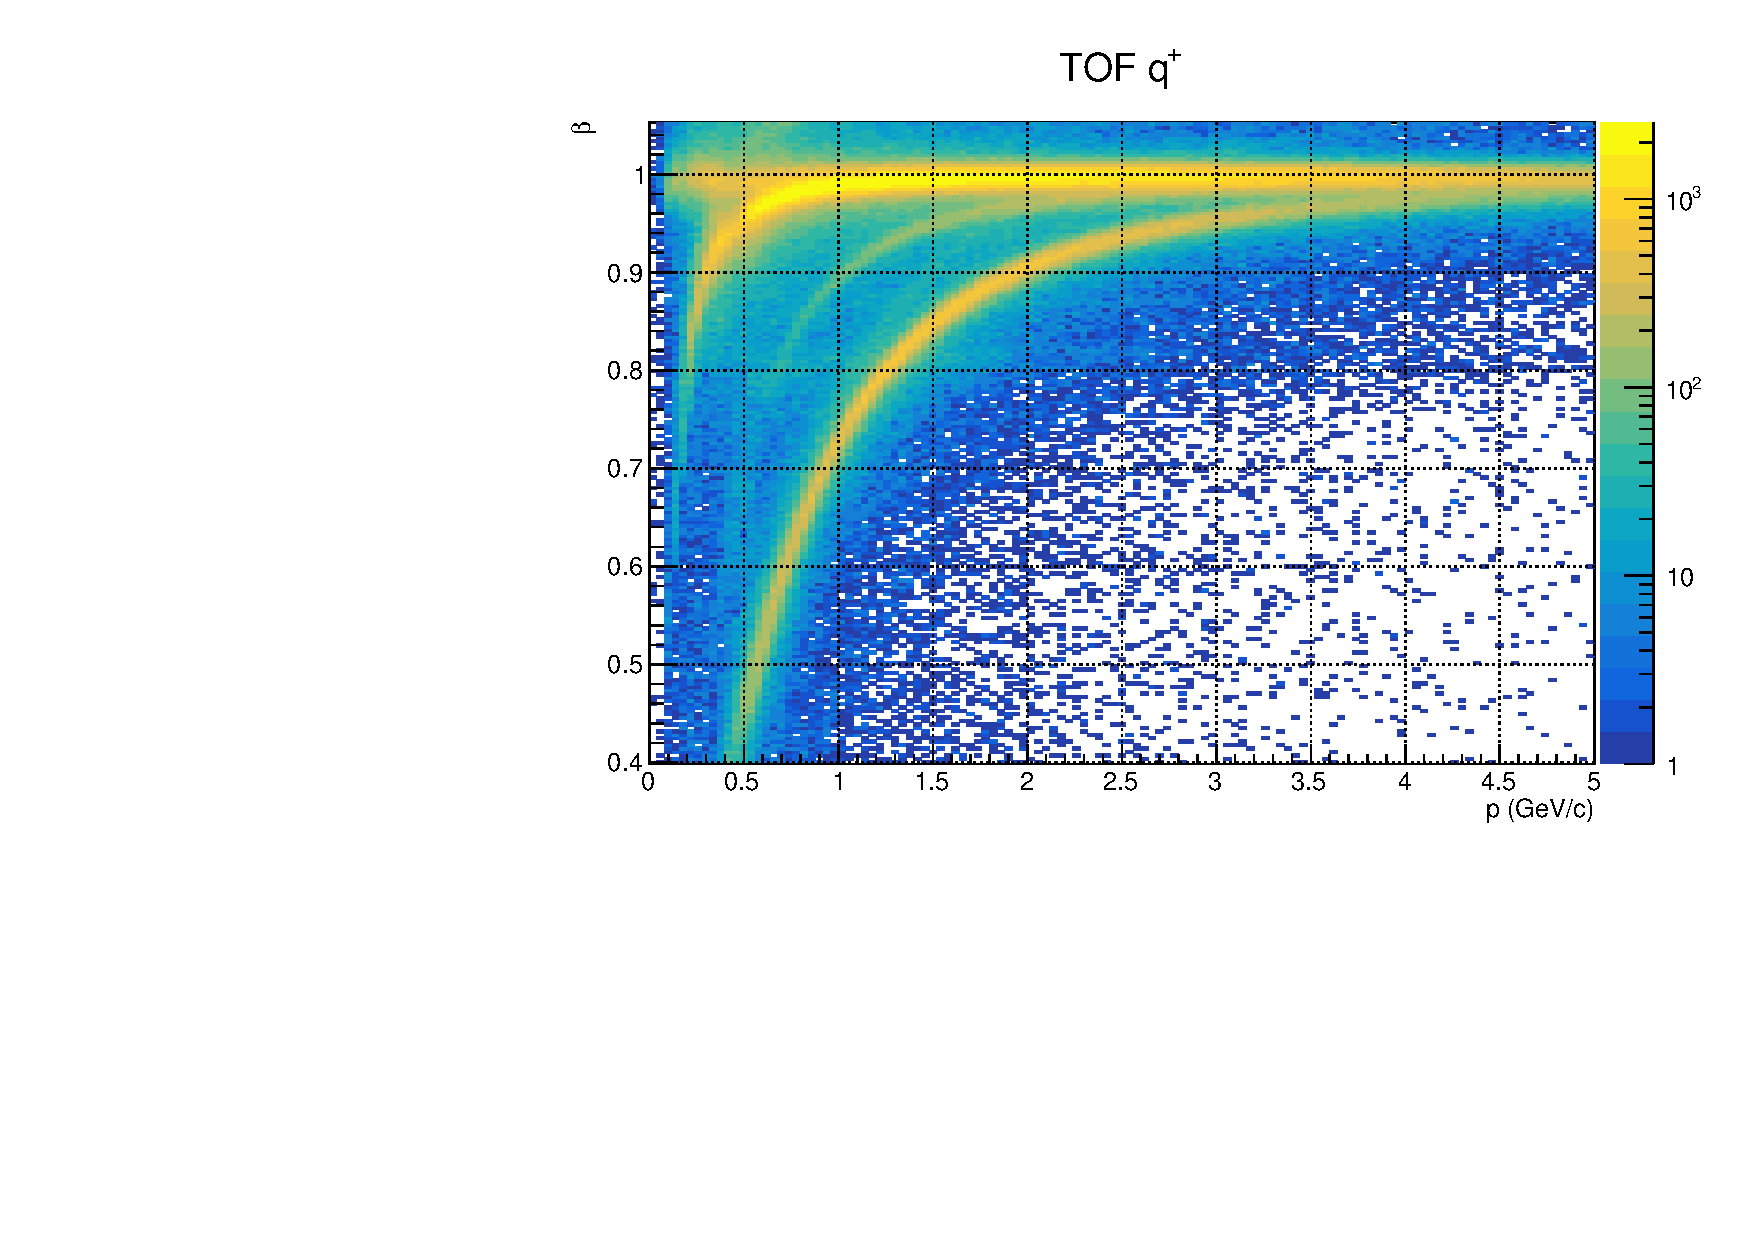
\includegraphics[width=0.6\textwidth]{figures/beta_vs_p_positivetracks.pdf}
\caption{\label{fig:betavsp}$\beta$ of positive charged tracks versus track momentum, showing obvious bands for $e^+$, $\pi^+$, $K^+$ and $p$. The color coding of the third dimension
is in logarithmic scale.(Color online)}
\end{center}
\end{figure}

\begin{figure}[tbp]
\begin{center}
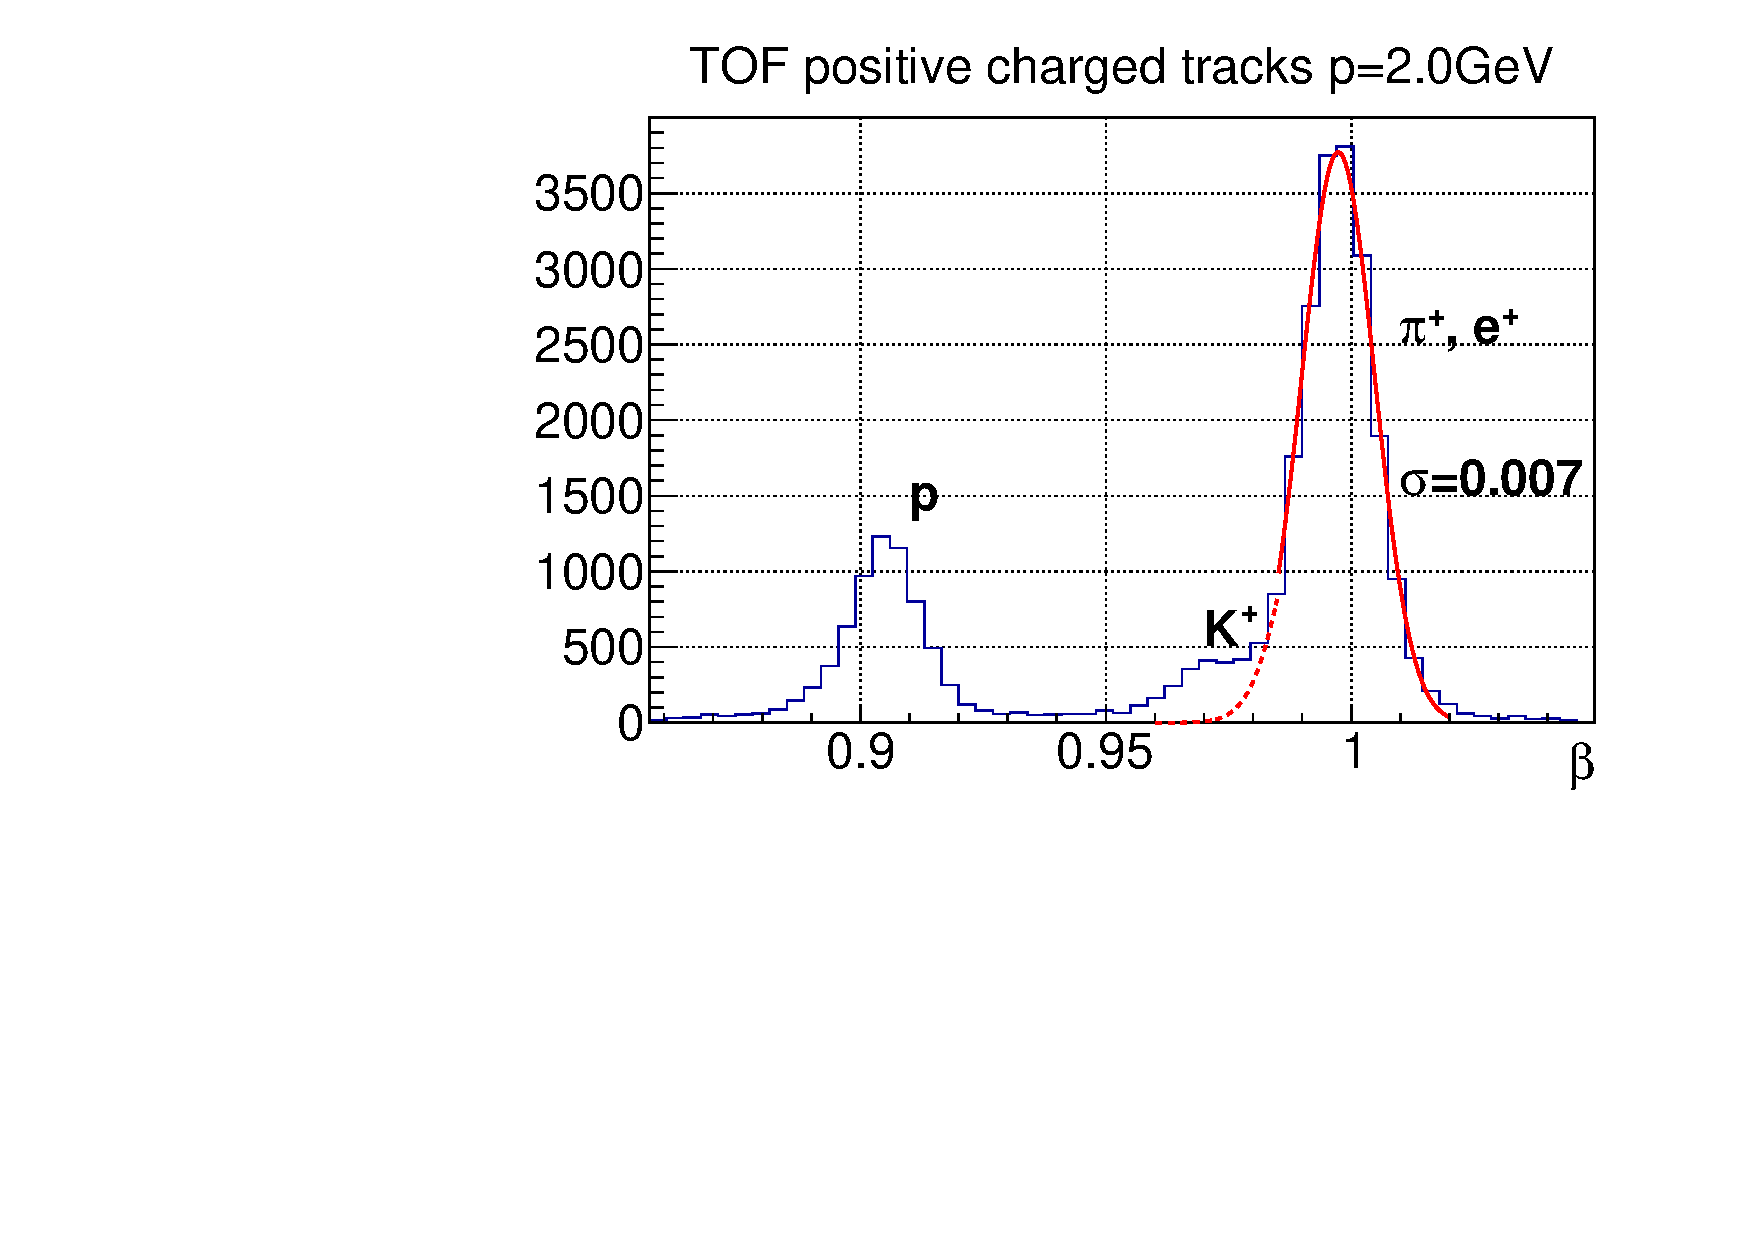
\includegraphics[width=0.45\textwidth]{figures/TOF_postracks_2000mev.pdf}
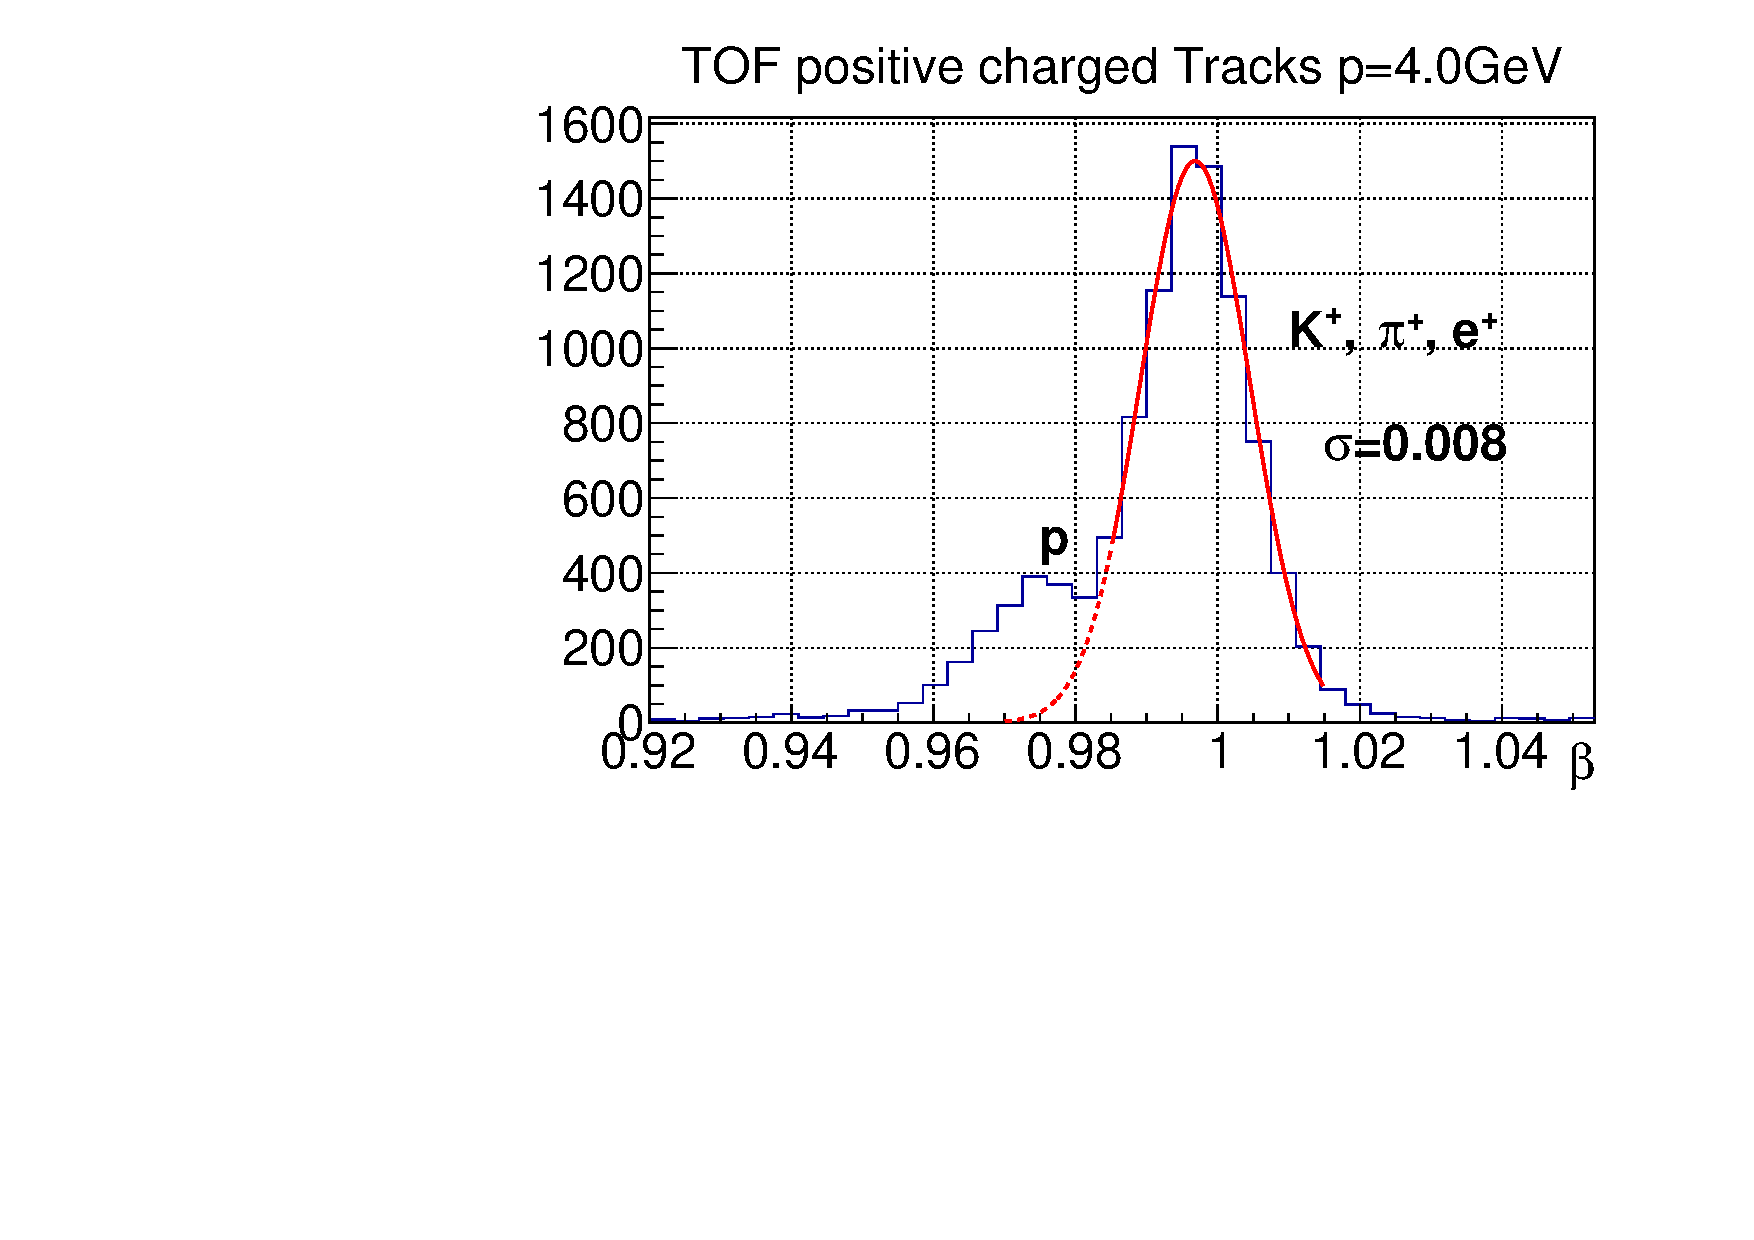
\includegraphics[width=0.45\textwidth]{figures/TOF_postracks_4000mev.pdf}
\caption{\label{fig:betaproj}$\beta$ of positive charged tracks with 2~GeV/c momentum (left) and with 4~GeV/c (right).}
\end{center}
\end{figure}
